\section{Krzysztof's Chapter}

Below, you will find some digits of $\pi$, if that is what you desire. If that is not what you desire, you will find there digits of $\pi$ anyway, because that is just simpler.

\begin{table}[h!]
\begin{center}
    \begin{tabular}{l|l|l|l}
    1 & 4 & 1 & 5 \\ \hline
    9 & 2 & 6 & 5
    \end{tabular}
    \caption{First 8 digits of pi (yes, I am a man of culture and subtlety).}
\end{center}
\end{table}

As an \textbf{intelligent}, \underline{culturally aware} person yourself, you will most probably \emph{dare} to ask what the meaning of the elephant image below is (see figure \ref{fig:elephant}). I must tell you -- I do not know, nor do I want to.

\begin{figure}[h!]
    \begin{center}
    \label{fig:elephant}
    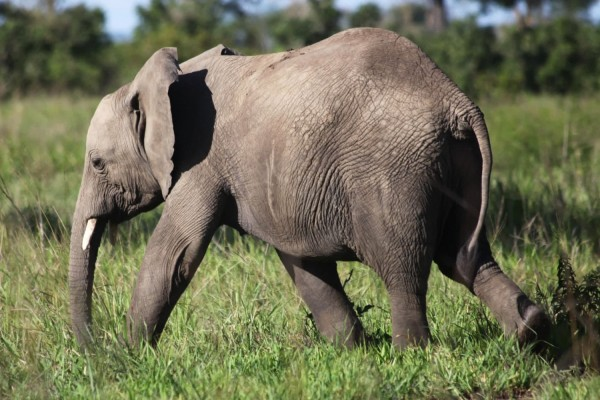
\includegraphics[width=0.6\textwidth]{Pictures/elephant.jpg}
    \caption{This is just some elephant}
    \end{center}
\end{figure}

Nevertheless, if you treat it as a variable, its meaning slowly unveils, as $\frac{\text{elephant}}{\text{elephant}^2} = \frac{1}{\text{elephant}}$. Furthermore:
\begin{equation}
    \lim_{\text{elephant}\to1} {\text{elephant}} = 1.
\end{equation}

Well, I have to admit I have not told you the whole truth about that elephant. It is not a variable, it is a \textbf{constant}. But I will give you a couple of hints about what that elephant could be:
\begin{itemize}
    \item $\text{Elephant} = 1$
    \item[!] $\text{Elephant} = 2$
    \item $\text{Elephant} = 3$
    \item[NOTE] $\text{Elephant} = 4$
\end{itemize}

If you still do not know:
\begin{enumerate}
    \item 2 is the first digit.
    \item Add $\pi$ to $e$.
    \item Subtract $\pi$.
\end{enumerate}

\begin{center}
Yes, that elephant was Mr. Euler all along.
\end{center}